\vvv\vvv\vvv
\presec
\subsection{Finding Persistent Items} \postsec
\label{sec:basicAlgorithm:persistent}

{\color{reviewD}
\ppp{Data Structure:}
The data structure of \aname{} of finding persistent items is exactly the same as that of our framework (Section \ref{sub:findinterest}): a Bloom filter and a min-heap. 
%The Bloom filter is used to remove duplicates in each period. 
%Each node of the min-heap stores an item ID and the corresponding persistency. 
%The root node stores the item with the smallest persistency. 
}


{\color{reviewD}
\ppp{Insertion:}
The insertion process of finding persistent items is similar to that of our Framework (see Section \ref{sub:findinterest}).
Here Bloom filter is used to check whether the item has probably been recorded in the current period.
The only difference is that we need to periodically empty the Bloom filter in this task.
%Given an incoming item, we first check the Bloom filter by calculating the $d$ hash functions. If the $d$ hashed bits are all 1, indicating that the item has probably been recorded in this period, we just discard the item. If the $d$ hashed bits are not all 1, we first set all the $d$ bits to 1. 
%
%Then, there are two cases: 1) If the item is in the min-heap, we increment the corresponding persistency by one. 2) Otherwise, the item is not in the min-heap, and if the min-heap is not full, we insert this item into the min-heap. If the min-heap is full, we try to insert the item into the root node using our PRI algorithm.
}


\ppp{Periodically Emptying:}
At the end of each period, we empty the Bloom filter by setting all bits to 0. In other words, the Bloom filter is used to indicate whether an item appears in the current period only.


{\color{reviewD}
\ppp{Report:}
The process of reporting persistent items is exactly the same as that of our framework (Section \ref{sub:findinterest}).
%To report all the items above a given threshold $\mathcal{T}$, we traverse the min-heap to pick out the items with persistencies larger than $\mathcal{T}$.
}

\begin{comment}

\begin{figure}[htbp]
	\centering
	\prefig
	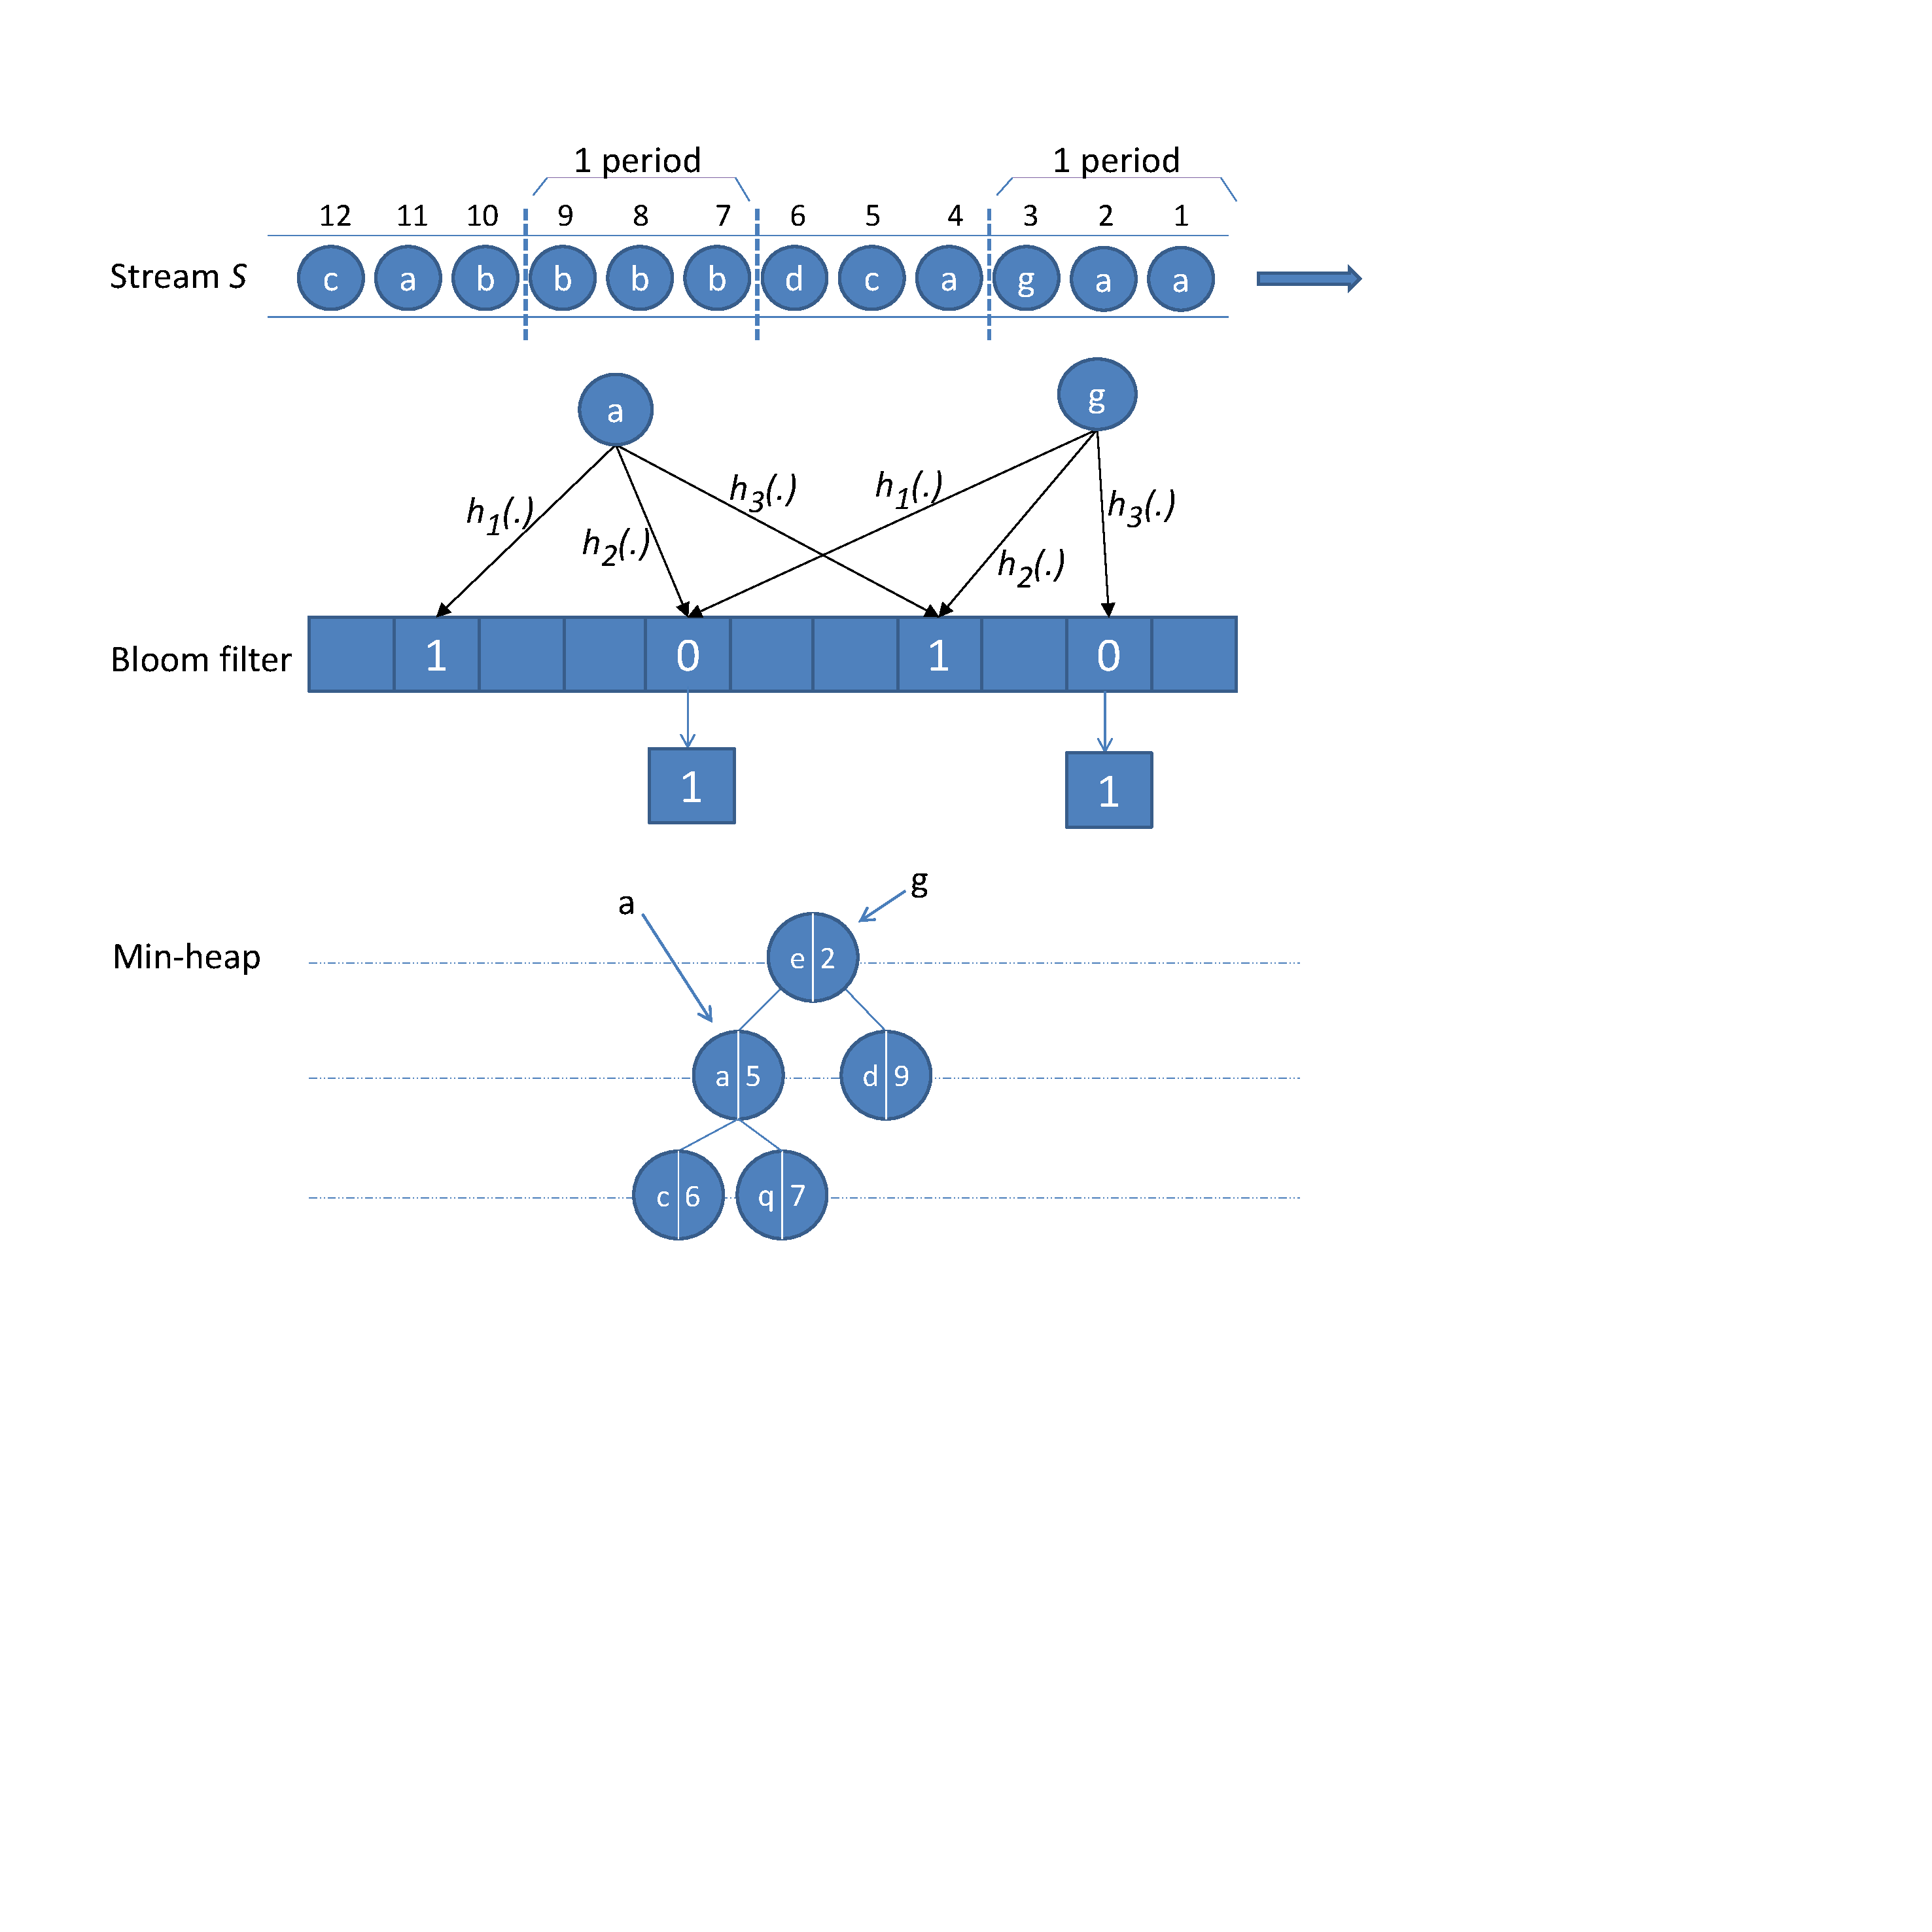
\includegraphics[width=0.5\textwidth]{example_per}
	\prefigcaption\vvv\vvv
	\caption{\aname{} for finding persistent items.}
	\label{draw:persistency}
	\postfig \vvv\vvv
\end{figure}

\ppp{Example:}
As shown in Figure \ref{draw:persistency}, for a given data stream, we divide them into multiple equal-sized periods. 
%
For the first incoming item $a$, we get the three hashed bits ($1,0,1$), which means that item $a$ has not been recorded in the min-heap in this period. 
%
Therefore, we change the hashed bit from $0$ to $1$ in the Bloom filter and increment the persistency of $a$ by one in the min-heap. 
%
Next we calculate three hash functions $h_1(a),h_2(a),h_3(a)$ for the second incoming item $a$. 
%
The three hashed bits are all $1$, which indicates that $a$ has been recorded in this period and thus the second item $a$ is discarded. 
%
When the third item $g$ arrives, the third hashed bit is $0$, so we insert $g$ into the min-heap and change the third hashed bit from $0$ to $1$.
%
Since $g$ is not in the min-heap, we try to insert it into the root node by applying our PRI algorithm. 
%
At the end of each period, we empty the Bloom filter by setting all bits to $0$. 
%
In this way, when the fourth item $a$ arrives in the next period, the persistency of $a$ in the min-heap can be incremented by one regardless of the record in the previous period.
\end{comment}

%
%The algorithm is shown in Algorithm~\ref{alg:per} in Appendix~\ref{sec:appendix}.
%
%The detailed description of the algorithm is similar to Algorithm~\ref{alg:basic}.

\presub
\subsection{{\color{reviewD}For Hopping Windows and Sliding Windows}}
\postsub


{\color{reviewD}
Our algorithm can also be used for hopping windows and sliding windows.
%handle the problems with a small change. 
As for hopping windows, we need a InterestSketch for each window. As for the overlap between the windows, an item may need to be checked in many InterestSketchs. Once a window runs out of time, the InterestSketch should be immediately set to zero, and it can be used for a new window. Therefore, the memory overhead will be $k-1$ more InterestSketch than the original algorithm. The sliding window is a special case of hopping window with a very large $k$. We also can handle the sliding window with more memory overhead.}



\vvv
\presub
\subsection{Shortcomings of the Basic Version}
\postsub

Our basic version has the following two shortcomings.
%
%First, when judging whether an item is in the min-heap, the whole heap should be traversed with the time complexity of $O(k)$, where $k$ is the number of items in the min-heap. 
%
First, we need to check whether every incoming item is in the min-heap, and the time complexity is $O(k)$, where $k$ is the number of items in the min-heap. 
%
This problem can be solved by adding a hash table. However, the hash table will inevitably bring hash collisions and a waste of memory space. 
%
Second, when updating the min-heap, the time complexity is $O(logk)$. Since the speed of data streams is often high, we wish to reduce the time complexity from $O(logk)$ to $O(1)$.